% Makros zur Kompatibilitaet mit Onlinemodul: 
 \providecommand{\MoIl}[1][]{\mbox{}#1]\mathopen{}} 
 \providecommand{\MoIr}[1][]{#1[\mbox{}} 
 \providecommand{\MIntvlSep}{;} 
 \providecommand{\MElSetSep}{\, ; \, } 
 \begin{MAufgabe}{Lineare Betrags(un)gleichungen}{vr, 2016, MaTeX}
L\"osen Sie die Gleichung
$$
 \MDS 3\left| 8\, x + 4 \right|+x + 1=  \left| 1 - 2\, x \right|  - x - 1
$$  

\ifLsg\MLoesung

Im ersten Schritt k\"onnen die Terme au\ss{}erhalb der Betragszeichen zusammengefasst werden:

\begin{align*} 
 3\left| 8\, x + 4 \right|+x + 1=  \left| 1 - 2\, x \right|  - x - 1\\ 
\Leftrightarrow2\, x - \left|2\, x - 1\right| + 3\, \left|8\, x + 4\right| + 2= 0 
 \end{align*}

F\"ur diese Gleichung haben wir 4 F\"alle zu unterscheiden: 
\begin{enumerate}
\item $ \MDS 
\begin{cases} 
 0 \leq 8\, x + 4\\ 
0 \leq 1 - 2\, x
 \end{cases}
\Leftrightarrow - \frac{1}{2} \leq x \wedge x \leq \frac{1}{2}\Leftrightarrow x \in [ - \frac{1}{2} \, \MIntvlSep \, \frac{1}{2}]$ 
\item $ \MDS 
\begin{cases} 
 0 \leq 8\, x + 4\\ 
1 - 2\, x < 0
 \end{cases}
\Leftrightarrow \frac{1}{2} < x\Leftrightarrow x \in \MoIl  \frac{1}{2} \, \MIntvlSep \, \infty\MoIr $ 
\item $ \MDS 
\begin{cases} 
 8\, x + 4 < 0\\ 
0 \leq 1 - 2\, x
 \end{cases}
\Leftrightarrow x < - \frac{1}{2}\Leftrightarrow x \in \MoIl  -\infty \, \MIntvlSep \, - \frac{1}{2}\MoIr $ 
\item $ \MDS 
\begin{cases} 
 8\, x + 4 < 0\\ 
1 - 2\, x < 0
 \end{cases}
 \mbox{ : keine L\"osung. Diese Bedingung ist nirgendwo erf\"ullt.}$ 
\end{enumerate} 
Der 4. Fall ist nirgendwo erf\"ullt. Betrachte weiter nur die restlichen F\"alle.
 
 Fallunterscheidung: 

 \begin{enumerate} 
 \item Sei $ \MDS x\in[ - \frac{1}{2} \, \MIntvlSep \, \frac{1}{2}]$. 
 In diesem Fall gilt: 
  $ \MDS \left| 8\, x + 4\right|=8\, x + 4$ und $ \MDS \left| 1 - 2\, x\right|=1 - 2\, x$. \\ 
 Damit ist die Gleichung 
 $$ 
2\, x - \left|2\, x - 1\right| + 3\, \left|8\, x + 4\right| + 2= 0
$$
 \"aquivalent zur Gleichung
 $$ 
3\left(8\, x + 4\right)-\left( 1 - 2\, x\right)+2\, x+2= 0 
$$  
$$ 
 \Leftrightarrow 28\, x + 13= 0 
$$  
$$ \Leftrightarrow x = - \frac{13}{28} . 
 $$ 
 Die L\"osung muss auch die Fallbedingung $x\in [ - \frac{1}{2} \, \MIntvlSep \, \frac{1}{2}] $ erf\"ullen. Die gefundene L\"osung $x=- \frac{13}{28}$ erf\"ullt die Fallbedingung  $x\in [ - \frac{1}{2} \, \MIntvlSep \, \frac{1}{2}]$ und deshalb ist  $$
 \mathcal{L}_{1}=\left\{- \frac{13}{28}\right\}
 $$ 
\item Sei $ \MDS x\in\MoIl  \frac{1}{2} \, \MIntvlSep \, \infty\MoIr $. 
 In diesem Fall gilt: 
  $ \MDS \left| 8\, x + 4\right|=8\, x + 4$ und $ \MDS \left| 1 - 2\, x\right|=2\, x - 1$. \\ 
 Damit ist die Gleichung 
 $$ 
2\, x - \left|2\, x - 1\right| + 3\, \left|8\, x + 4\right| + 2= 0
$$
 \"aquivalent zur Gleichung
 $$ 
3\left(8\, x + 4\right)-\left( 2\, x - 1\right)+2\, x+2= 0 
$$  
$$ 
 \Leftrightarrow 24\, x + 15= 0 
$$  
$$ \Leftrightarrow x = - \frac{5}{8} . 
 $$ 
 Die L\"osung muss auch die Fallbedingung $x\in \MoIl  \frac{1}{2} \, \MIntvlSep \, \infty\MoIr  $ erf\"ullen. Die gefundene L\"osung $x=- \frac{5}{8}$ erf\"ullt die Fallbedingung  $x\in \MoIl  \frac{1}{2} \, \MIntvlSep \, \infty\MoIr $ nicht und deshalb ist  $$
 \mathcal{L}_{2}=\emptyset 
 $$ 
\item Sei $ \MDS x\in\MoIl  -\infty \, \MIntvlSep \, - \frac{1}{2}\MoIr $. 
 In diesem Fall gilt: 
  $ \MDS \left| 8\, x + 4\right|= - 8\, x - 4$ und $ \MDS \left| 1 - 2\, x\right|=1 - 2\, x$. \\ 
 Damit ist die Gleichung 
 $$ 
2\, x - \left|2\, x - 1\right| + 3\, \left|8\, x + 4\right| + 2= 0
$$
 \"aquivalent zur Gleichung
 $$ 
3\left( - 8\, x - 4\right)-\left( 1 - 2\, x\right)+2\, x+2= 0 
$$  
$$ 
 \Leftrightarrow  - 20\, x - 11= 0 
$$  
$$ \Leftrightarrow x = - \frac{11}{20} . 
 $$ 
 Die L\"osung muss auch die Fallbedingung $x\in \MoIl  -\infty \, \MIntvlSep \, - \frac{1}{2}\MoIr  $ erf\"ullen. Die gefundene L\"osung $x=- \frac{11}{20}$ erf\"ullt die Fallbedingung  $x\in \MoIl  -\infty \, \MIntvlSep \, - \frac{1}{2}\MoIr $ und deshalb ist  $$
 \mathcal{L}_{3}=\left\{- \frac{11}{20}\right\}
 $$ 
 \end{enumerate} 
  Die L\"osungsmenge des Ausgangsproblems ist die Vereinigung der einzelnen L\"osungsmengen: 
$$ \mathcal{L} = \mathcal{L}_{1} \cup \mathcal{L}_{2} \cup \mathcal{L}_{3} 
 = \left\{- \frac{13}{28}\right\}\cup \emptyset\cup \left\{- \frac{11}{20}\right\} 
  =\left\{- \frac{13}{28}\right\}\cup\left\{- \frac{11}{20}\right\} 
  = \left\{- \frac{13}{28}\MElSetSep- \frac{11}{20}\right\} 
 . $$ 
 
 \begin{center}
 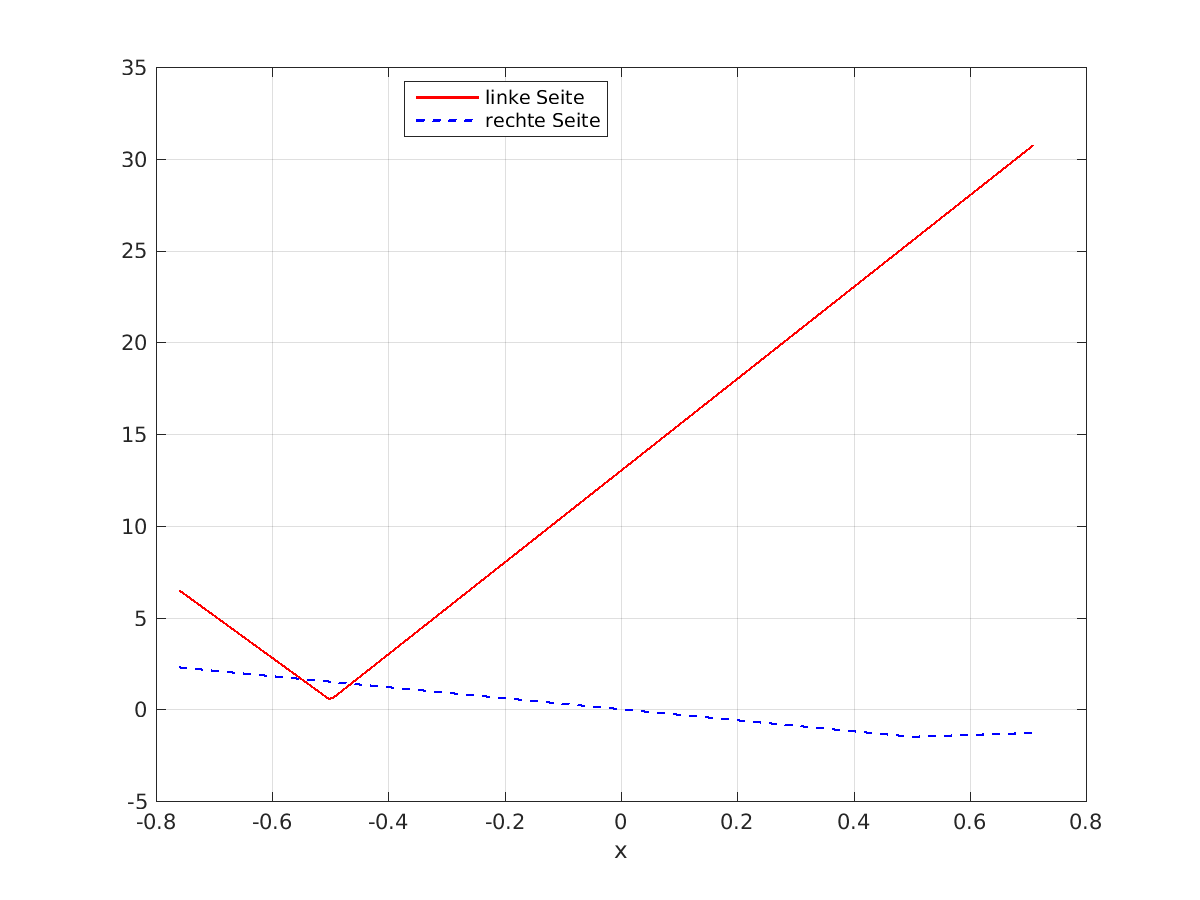
\includegraphics[width=0.8\linewidth]{Abb_zur_Ag_autogenerated_ineq_10.png} \end{center}
 
\else\relax\fi
 \end{MAufgabe}